\section{Results and Discussion}


Through tens of thousands experiments across many signal-processing techniques (\textit{e.g.}, defences), random states, learning rates, model architectures, and attack configurations, we show that model defences generally fail to outperform the undefended model in either the benign or adversarial contexts--- regardless of configuration; that the adversarial failure rate gains of larger ResNet configurations are driven by response time rather than true robustness; that these gains are dwarfed by the increase in training time; and that AFR models are a powerful tool for comparing model architectures and examining the effects of covariates. In the section below, we display and discuss the results for the CIFAR100, CIFAR10, and MNIST datasets for all attacks and defences. 

\subsection{Benign and Adversarial Accuracy}
\cm{
Fig.~\ref{fig:accuracies} depicts the benign and adversarial accuracies across the various attacks and defences. We can clearly see that no defence consistently outperforms the undefended (control) model in either the benign (top) or adversarial context (middle). We also see that for all defences, we can find at least one configuration with arbitrarily high accuracy, though finding it might involve an expensive hyper-parameter search as evidenced by the large variance (see top plot of Fig.~\ref{fig:accuracies}). Likewise, the adversarial accuracy benefits greatly from model tuning, but that attacks are still effective on roughly 75\% of samples in the best case for most attacks (see middle plot of Fig.~\ref{fig:accuracies}). Despite varying methods and computational costs, the attacks seem to be more or less equally effective with respect to adversarial accuracy (see bottom plot of Fig.~\ref{fig:accuracies}).
}


\label{results}
\begin{figure}[!h]
\begin{subfigure}
    \centering
    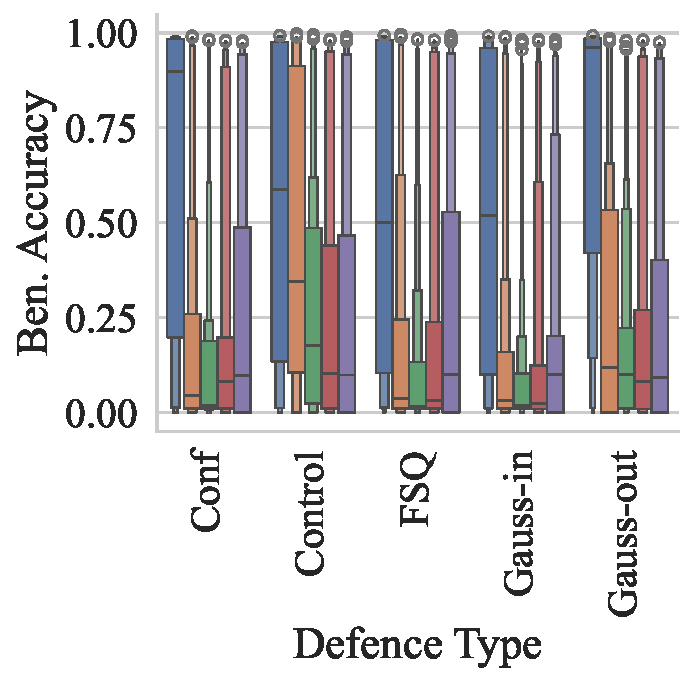
\includegraphics[trim={0 5pt 0 10pt},clip,width=.45\textwidth]{plots/ben_accuracy_vs_defence_type.pdf}
\end{subfigure}
\begin{subfigure}
    \centering
    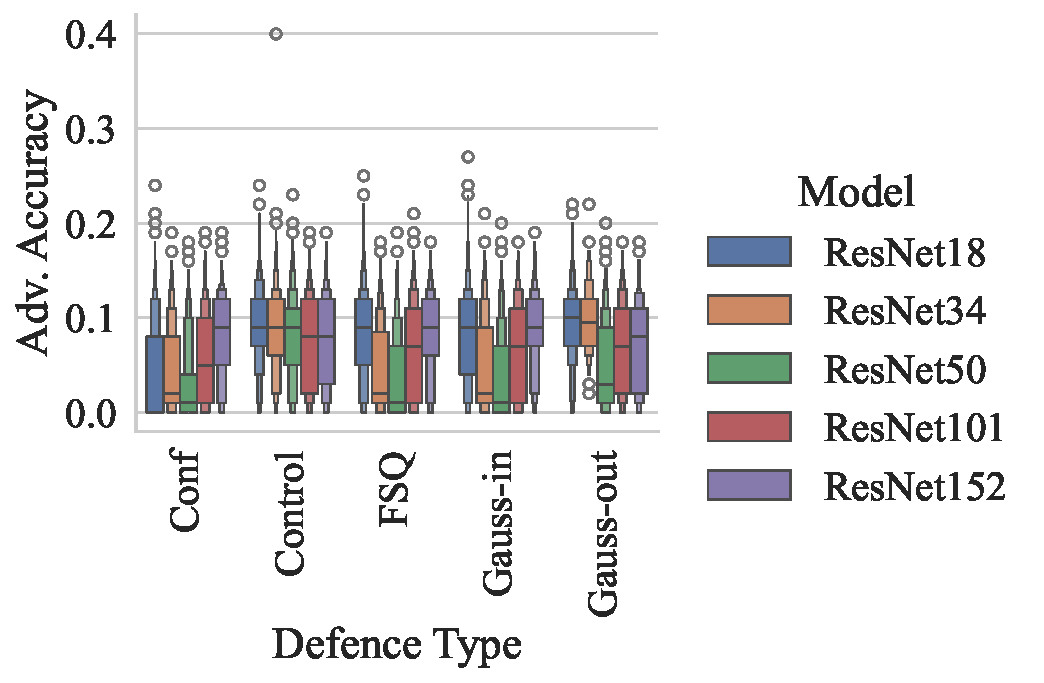
\includegraphics[trim={0 5pt 0 10pt},clip,width=.45\textwidth]{plots/adv_accuracy_vs_defence_type.pdf}
\end{subfigure}
\begin{subfigure}
    \centering
    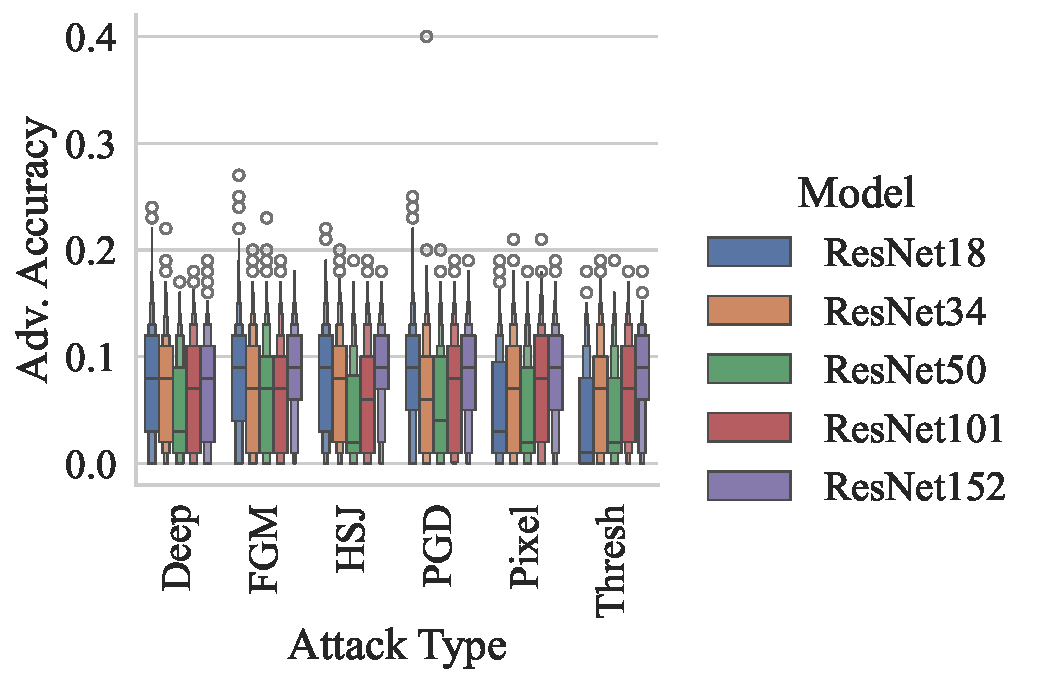
\includegraphics[trim={0 5pt 0 10pt},clip,width=.45\textwidth]{plots/adv_accuracy_vs_attack_type.pdf}
\end{subfigure}
\caption{The adversarial accuracy across various attacks pictured on the x-axis and outlined in Section~\ref{attacks}. The error bar reflects the 95\% confidence interval for the adversarial accuracy across all examined samples. The violin plots reflect the 95\% confidence intervals for each tuned hyperparameter combination. Outliers are indicated with a circle.}
\label{fig:accuracies}
\end{figure}



% \begin{figure}[!h]
%     \centering
%     \begin{subfigure}
%         \centering
%         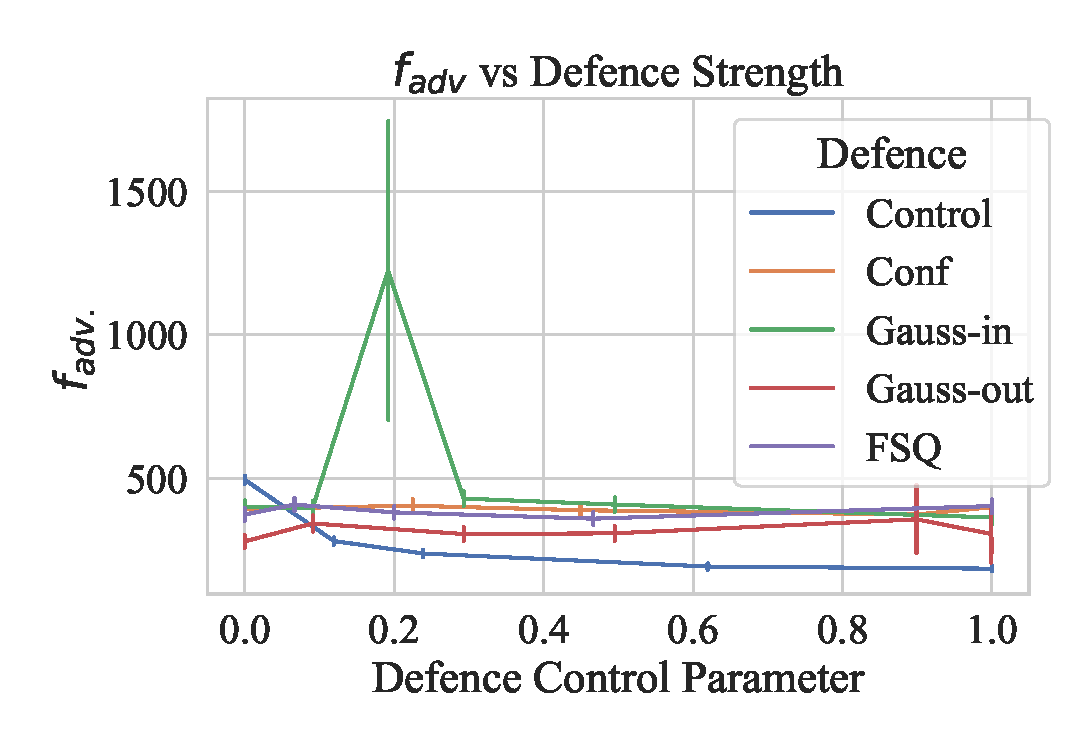
\includegraphics[width=.4\textwidth]{plots/def_param_vs_adv_failure_rate.pdf}
%     \end{subfigure}
%     \begin{subfigure}
%         \centering
%         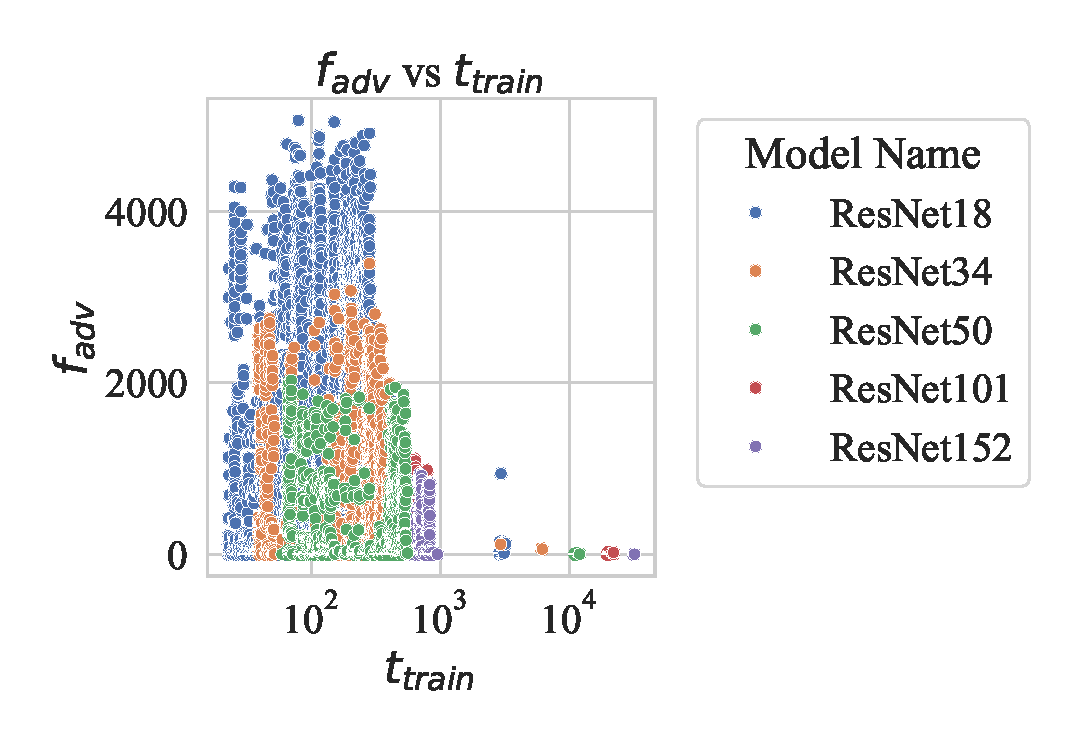
\includegraphics[width=.4\textwidth]{plots/adv_failure_rate_vs_train_time.pdf}
%     \end{subfigure}
%     \caption{The left shows the adversarial failure rate as a function of the defence strength where the control parameter represents the number of model layers. The right depicts the adversarial failure rate as a function of training time and the ResNet configuration. The bars indicate the first standard deviation of measures across all model configurations.}
%     \label{fig:failure_rate}
% \end{figure}






% \subsection{Attack and Defence Strength}
% In Fig.~\ref{fig:strength}, \cm{we can see the effect of the (min-max scaled) control parameter on the benign and adversarial accuracy}. Furthermore, the relationship between the defence control parameter and the benign accuracy is not monotonic, meaning that tuning is will be expensive. We can see that the relationship between the attack parameters and failure rate is also not monotonic. However, all defences appear to perform much worse in the average adversarial case (right) than in the benign (left). Additionally we see in the right side of Fig.~\ref{fig:strength} that the attack types yield relatively consistent results, with the mean of one falling in the 95 confidence intervals of all the others. We can also see that defence choice follows the same pattern, except for Gauss-in, which rapidly decreases the accuracy as we increase the input noise beyond some threshold in which accuracy tends to increase.

% \begin{figure}[!h]
%     \centering
%     \begin{subfigure}
%         \centering
%         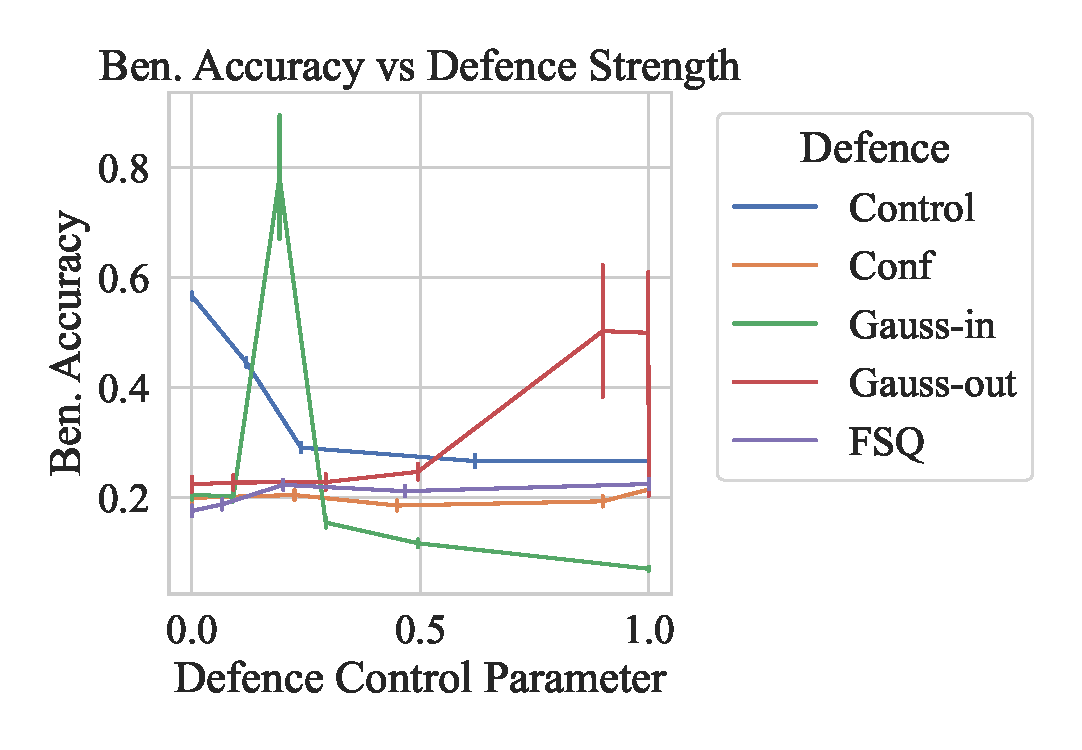
\includegraphics[trim={0 10pt 0 10pt},clip,width=.45\textwidth]{plots/def_param_vs_accuracy.pdf}
%     \end{subfigure}
%     \begin{subfigure}
%         \centering
%         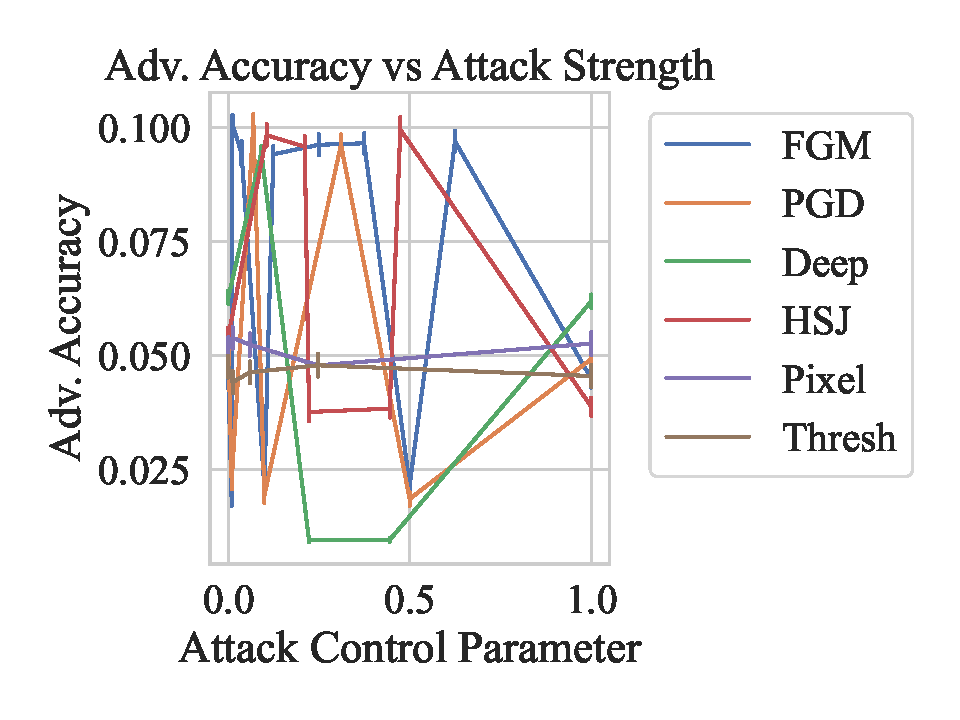
\includegraphics[trim={0 10pt 0 10pt},clip,width=.45\textwidth]{plots/atk_param_vs_accuracy.pdf}
%     \end{subfigure}
%     \caption{This depicts the benign (unperturbed) and adversarial (perturbed) failure rates across all defences attacks, and models. The left shows how the benign accuracy varies with the defence strength where the control parameter describes the number of layers. The right shows the adversarial accuracy as a function of attack strength. The bars indicate the first standard deviation of measures across all model configurations.}
%     \label{fig:strength}
% \end{figure}



\subsection{AFR Models}
\begin{table*}
\centering
\label{tab:afr_models}
\begin{tabular}{lllrrrrrr}
\toprule
 & AIC & BIC & Concordance & Test Concordance & ICI & Test ICI & E50 & Test E50 \\
\midrule
Cox & -- & -- & 0.92 & 0.92 & 0.06 & 0.27 & 0.04 & 0.08 \\
Gamma & -- & -- & 0.51 & 0.52 & 0.26 & 0.43 & 0.17 & 0.32 \\
Weibull & 9.05e+04 & 9.05e+04 & 0.92 & 0.92 & 0.02 & 0.2 & 0 & 0.01 \\
Exponential & 7.93e+04 & 7.93e+04 & 0.86 & 0.86 & 0.04 & 0.2 & 0 & 0.02 \\
Log Logistic & 9.79e+04 & 9.79e+04 & 0.92 & 0.92 & 0.07 & 0.08 & 0.01 & 0.01 \\
Log Normal & 1.14e+05 & 1.14e+05 & 0.91 & 0.91 & 0.15 & 0.26 & 0.08 & 0.19 \\
\bottomrule
\end{tabular}
\end{table*}

Table~\ref{tab:combined} contains the performance of each of these models on the CIFAR10 dataset. For all datasets, we can see that they are roughly comparable with regards to Concordance, but that log-logistic and exponential models marginally outperforms the other models when measured with AIC/BIC. Concordance is identical for both the test and train sets, with gamma and exponential falling behind the others. However, the ICI and E50 across the test train sets is superior for the Weibull, so we then used that model to infer the effect of the covariates (Fig.~\ref{fig:covariates}) as well as different attacks, defences, and datasets (Fig.~\ref{fig:dumies}). In that figure can clearly see that more hidden layers do increase the survival time. However, that seems to driven more by the model query time (see $t_predict$ in Fig.~\ref{fig:covariates}) than the number of model layers.

\begin{figure*}
	% \centering
	\begin{subfigure}
		\centering
		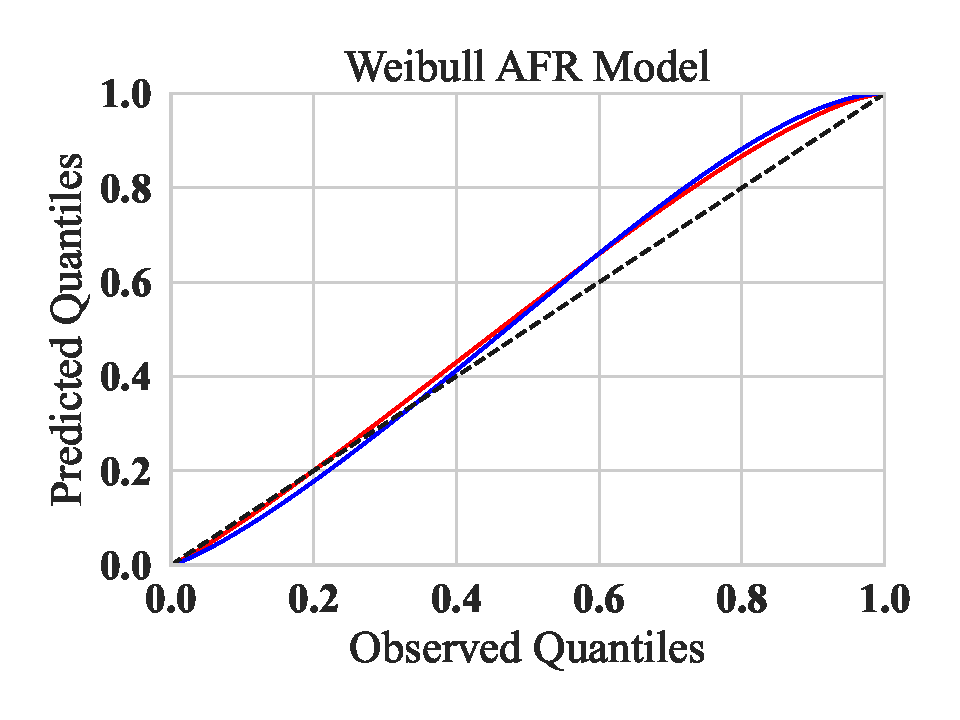
\includegraphics[width=.32\textwidth]{plots/weibull_qq.pdf}
	\end{subfigure}%
	~
	\begin{subfigure}
		\centering
		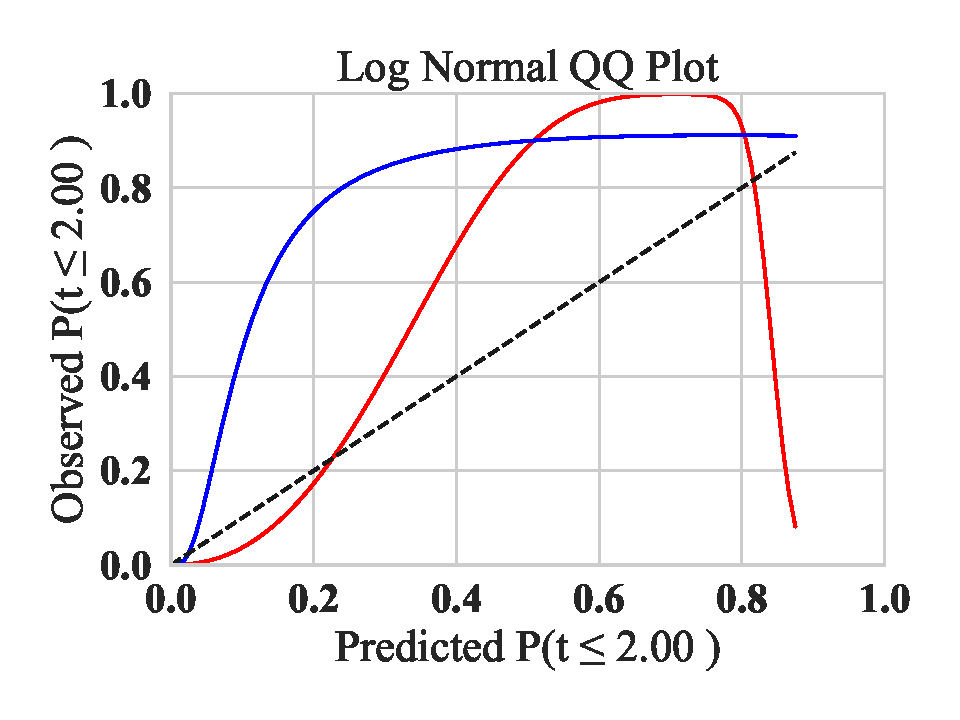
\includegraphics[width=.32\textwidth]{plots/log_normal_qq.pdf}
	\end{subfigure}
	~
	\begin{subfigure}
		\centering
		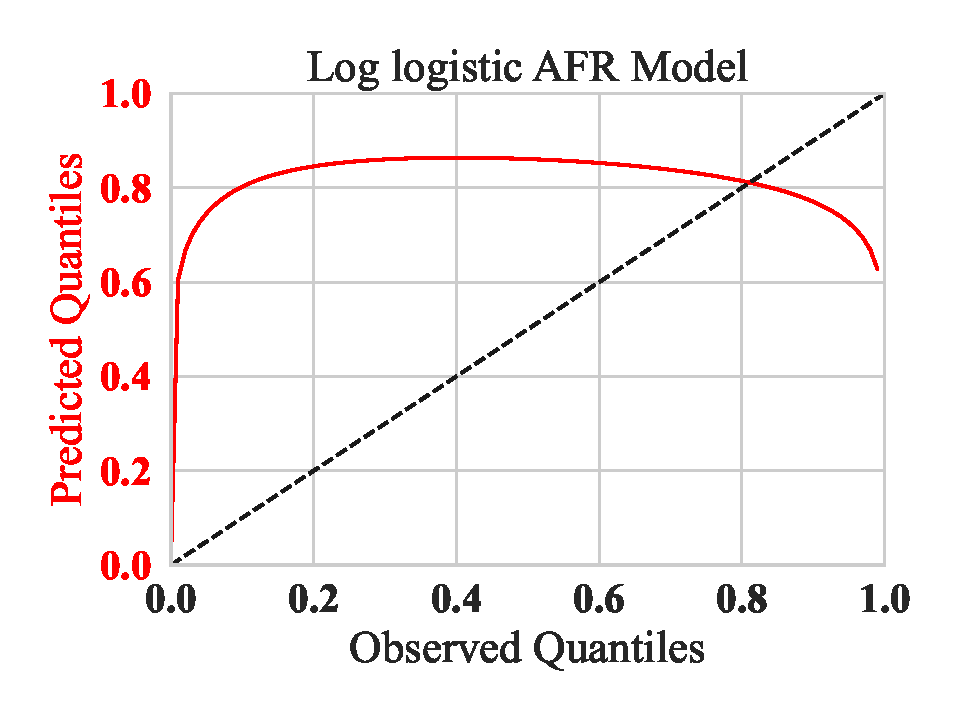
\includegraphics[width=.32\textwidth]{plots/log_logistic_qq.pdf}
	\end{subfigure}
 \begin{subfigure}
		\centering
		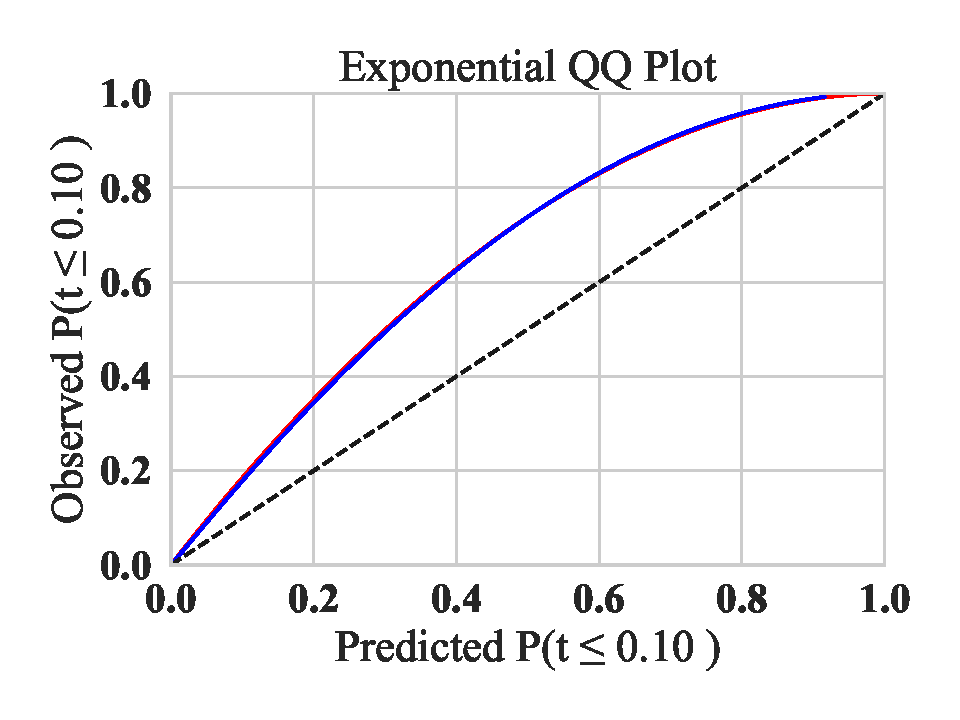
\includegraphics[width=.32\textwidth]{plots/exponential_qq.pdf}
	\end{subfigure}%
	~
	\begin{subfigure}
		\centering
		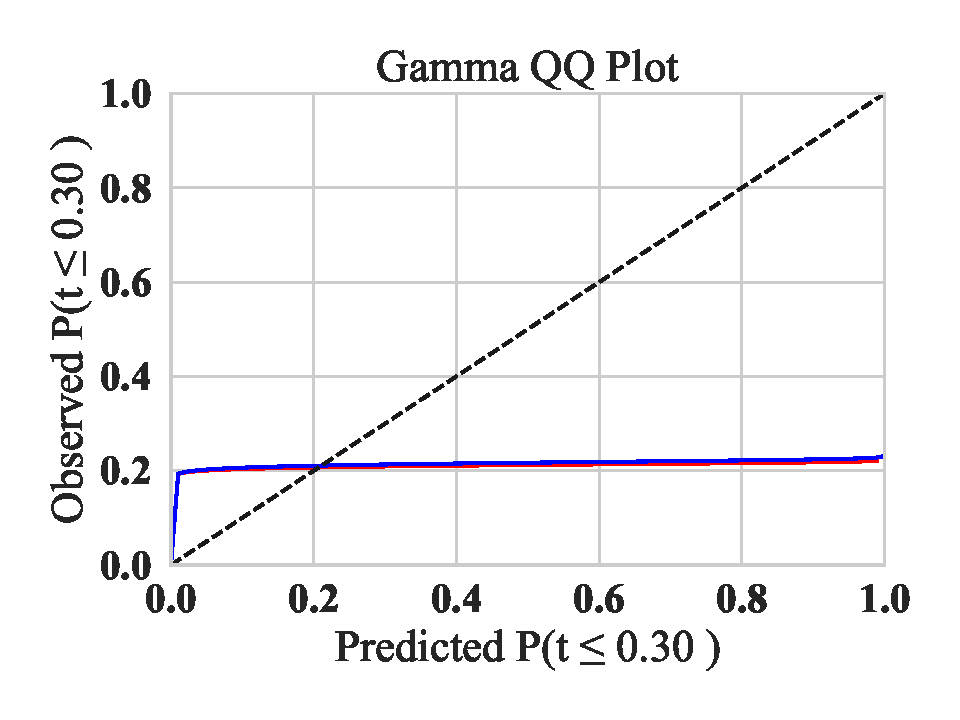
\includegraphics[width=.32\textwidth]{plots/gamma_qq.pdf}
	\end{subfigure}
	~
	\begin{subfigure}
		\centering
		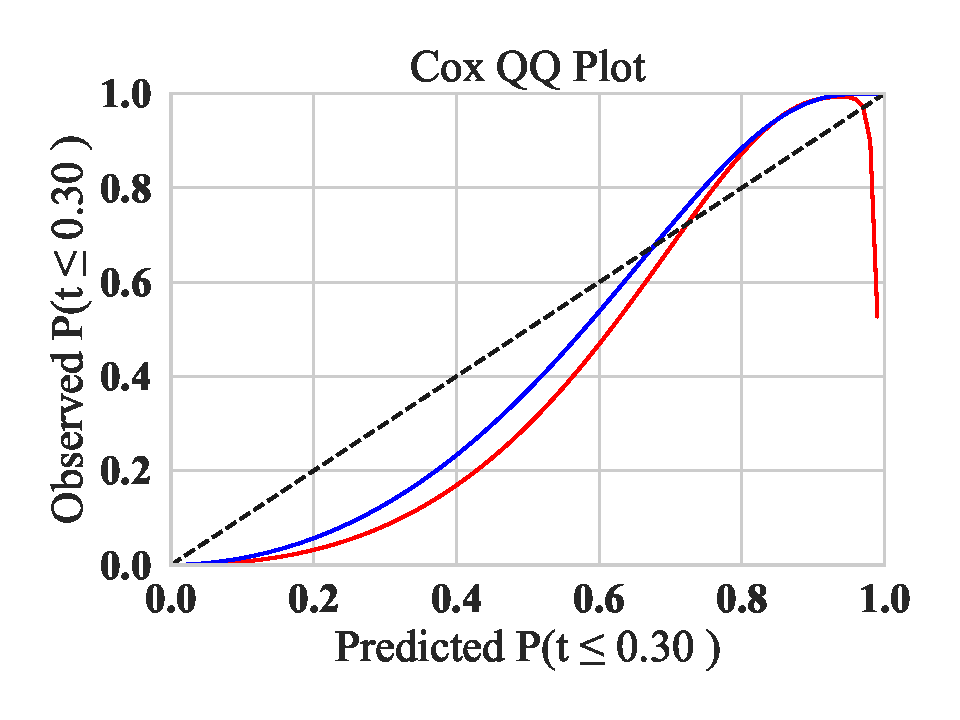
\includegraphics[width=.32\textwidth]{plots/cox_qq.pdf}
	\end{subfigure}
	\caption{These quantile-quantile plots demonstrate the efficacy of various AFR models. The first axis is the observed quantile of a sample and the second axis represents the theoretical quantile according to the chosen AFR model. The dashed black line represents a perfect fit. To verify each model, we reserved 80\% of the data to be the training set (blue) and 20\% to be the test set (red). 
 % The absence of one of the lines means that the \texttt{lifelines} fitter failed to converge for that subset.
 }
	\label{fig:afr_models}
\end{figure*}

\subsection{Effect of Covariates}
Fig.~\ref{fig:dummies} depicts the effect of all attacks, defences, and model configurations on the survival time and Fig.~\ref{fig:covariates} depicts the effect of the covariates. 
Fig.~\ref{fig:covariates} clearly demonstrates that increasing the depth of the model architecture does little for adversarial robustness while universally increasing the training time. 
Furthermore, it reveals something surprising---that increasing the number of epochs tends to increase the failure rate---even across model architectures and all defences. 
Certain defences can outperform the control model---at the cost of expensive tuning---evidenced by the large variance in performance (see Fig.~\ref{fig:dummies}). The scale of $t_train$  in Fig.~\ref{fig:covariates} shows that there is no general relationship between training time and adversarial survival time. \cm{Additionally, we see that an increase in accuracy tends to correspond to a decrease in survival time, confirming the inverse relationship noted by many researchers ~\cite{carlini_towards_2017,biggio_evasion_2013,croce_reliable_2020}.}
As the training time increases, however, the variance of attack times decreases, likely due to the corresponding increase in inference time (see:~\ref{fig:covariates}) rather than inherent robustness.
We formalize this analysis  in the next subsection.

\begin{figure}
    \centering
	\begin{subfigure}
	\centering
    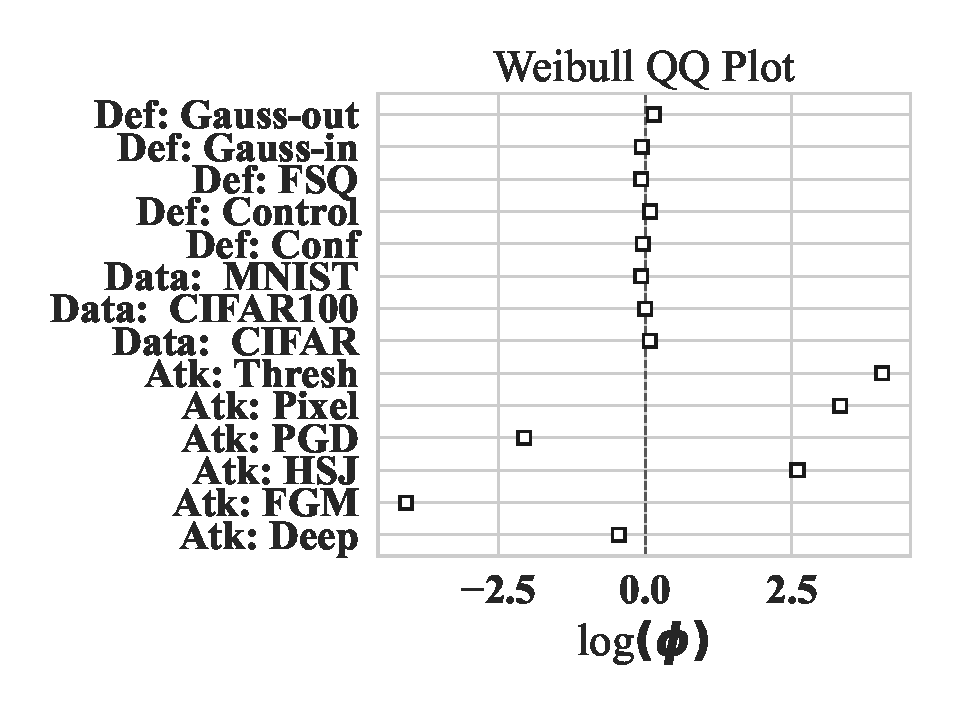
\includegraphics[width=.38\textwidth]{plots/weibull_aft_dummies.pdf}
    \label{fig:covariates}
    \end{subfigure}
    \begin{subfigure}
	\centering
    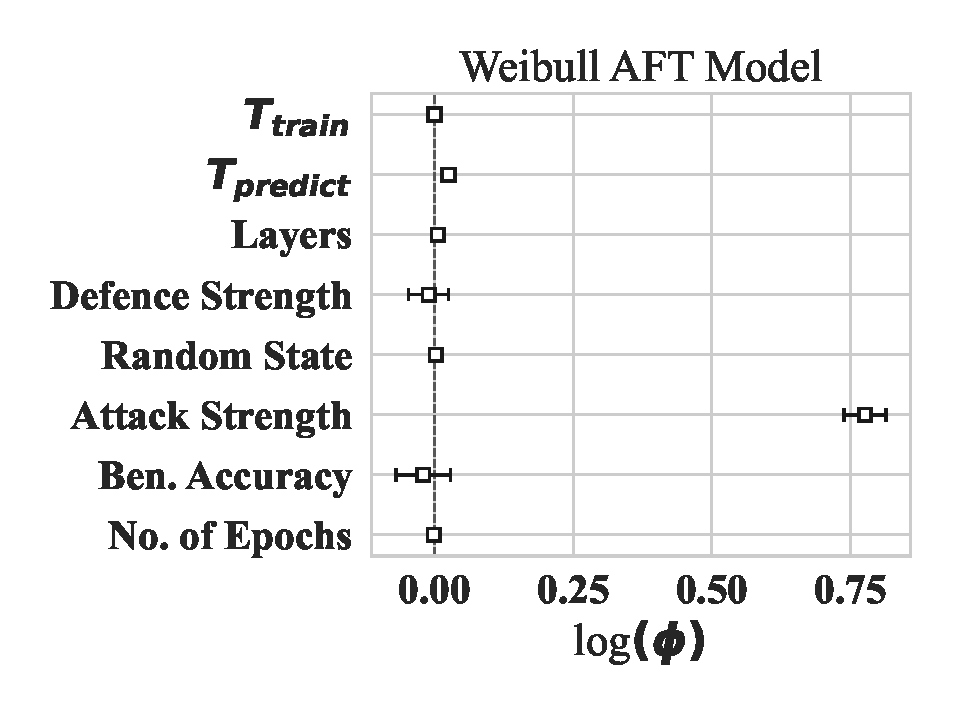
\includegraphics[width=.38\textwidth]{plots/weibull_aft.pdf}
    \label{fig:dummies}
    \end{subfigure}
    \caption{The coefficients represent the log scale effect of the dummy variables for dataset, attack, and defence on the survival time, with a positive value indicating an increase in the survival time.}
\end{figure}

\subsection{Failures and Cost}


Fig.~\ref{fig:failures_per_train_time} depicts the cost-normalized failure rate in both the benign (top) figure and adversarial cases (middle and bottom figures), using the Weibull model to calculate $\mathbb{E}_{S_\theta}$. Counter-intuitively, we see that the smallest model (ResNet18) tends to outperform both larger models (ResNet50 and ResNet152). Furthermore, we see that defence tuning is about as important as choosing the right type of defence (see: left side of Fig.~\ref{fig:failures_per_train_time}), with all defences falling within the normal ranges of each other. However, adding noise to the model output (Gauss-out) tends to underperform relative to the control for all models (see left side of Fig.~\ref{fig:failures_per_train_time}). Likewise, the intersectional relationship between model choice and optimal defence is highlighted since the efficacy of a defence depends as much on model architecture as it does on hyperparameter tuning.  Furthermore, performance across all attacks is remarkably consistent with intra-class variation being smaller than inter-class variation almost universally across defences and model configurations. \cm{Finally- and most importantly- we see that, while there is at least one configuration of each Resnet model that is cheaper to train than to fool in the benign context, that every single tested configuration costs orders of magnitude more to train than they do to attack with the Deep, FGM, or PGD attacks.}

\begin{figure}[!h]
    \centering
    \begin{subfigure}
        \centering
        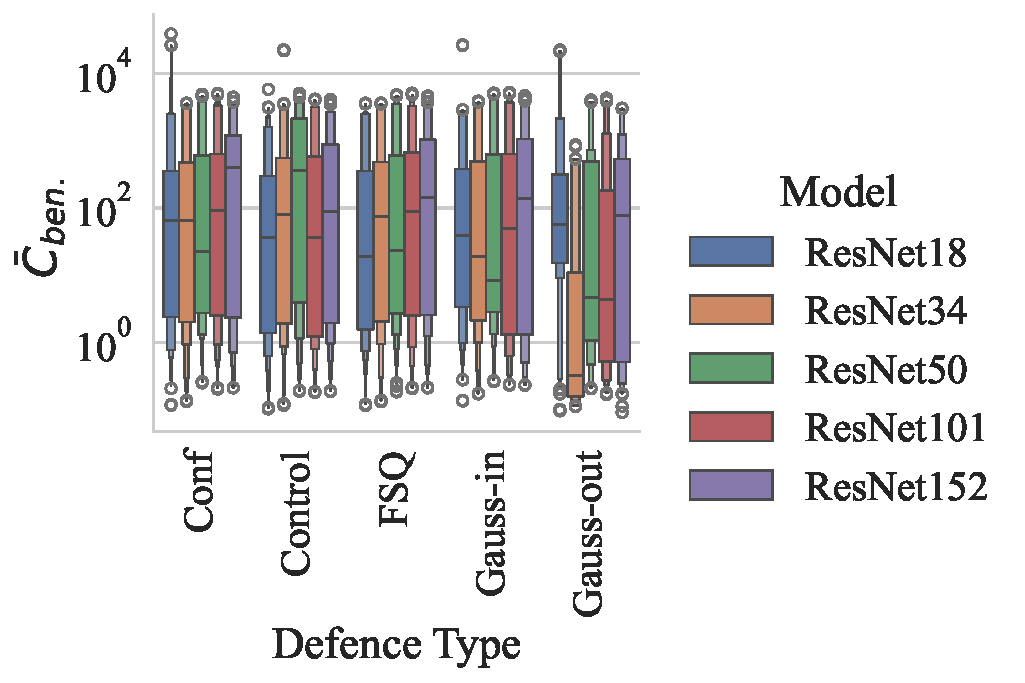
\includegraphics[width=.45\textwidth]{plots/ben_failures_per_train_time_vs_defence_type.pdf}
    \end{subfigure}
    \begin{subfigure}
        \centering
        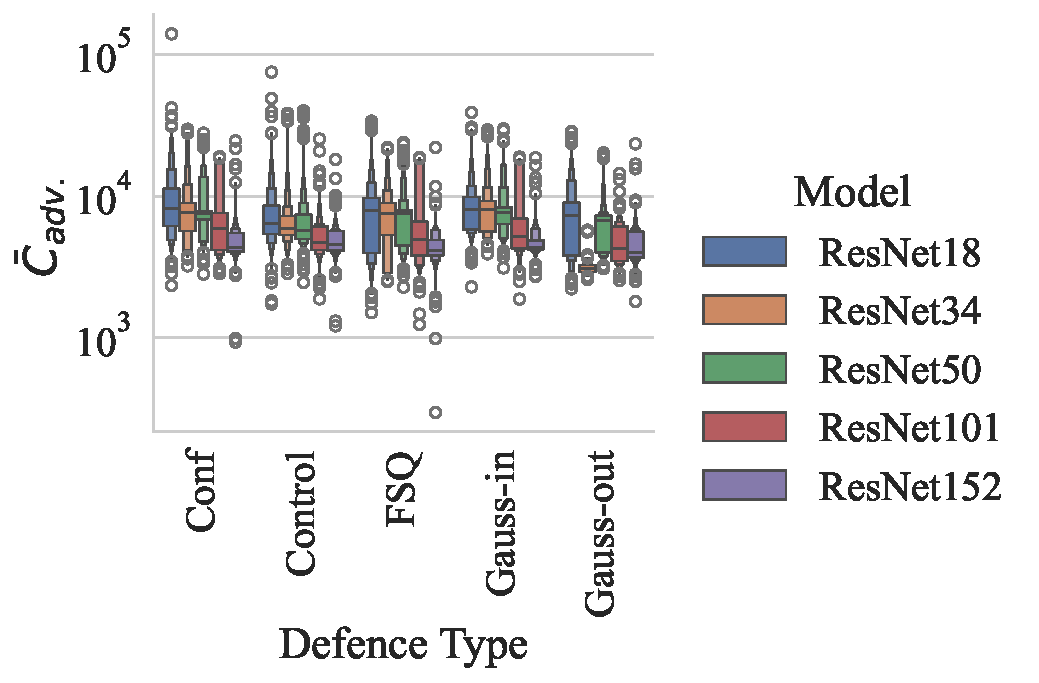
\includegraphics[width=.45\textwidth]{plots/adv_failures_per_train_time_vs_defence_type.pdf}
    \end{subfigure}
    \begin{subfigure}
        \centering
        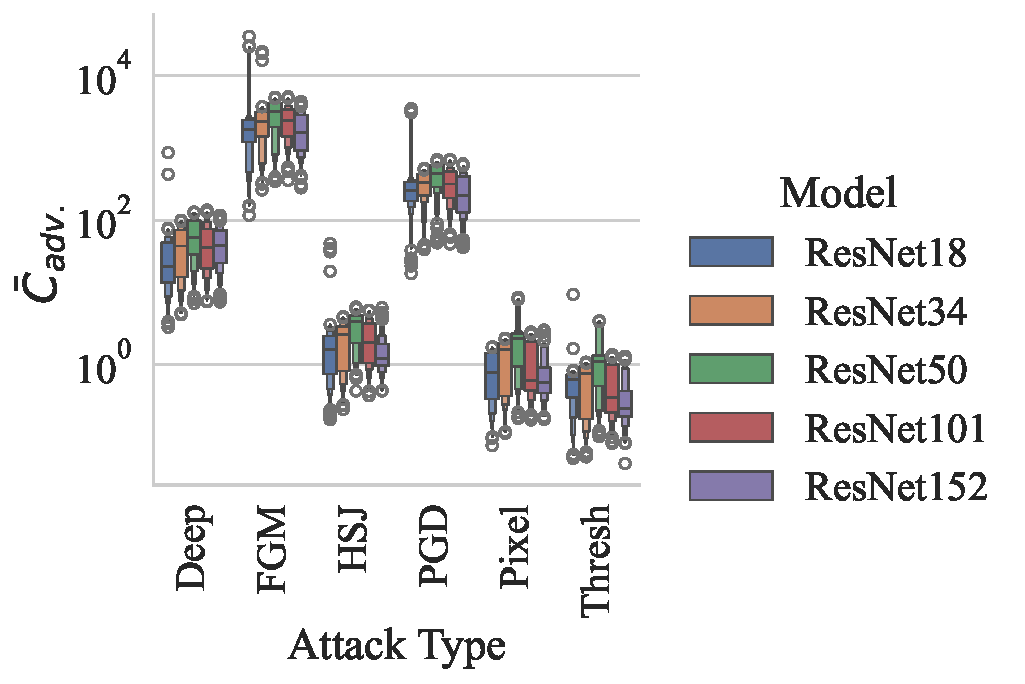
\includegraphics[width=.45\textwidth]{plots/adv_failures_per_train_time_vs_attack_type.pdf}
    \end{subfigure}
    \caption{This figure depicts the cost-normalized adversarial failure rate across a variety of defences and attacks, where training time (middle~\&~right Figs.) and inference time (left figure) is a stand-in for cost (see Section~\ref{cost}). The violin plots reflect the 95\% confidence intervals for each tuned hyperparameter combination. Outliers are indicated with a circle.}
    \label{fig:failures_per_train_time}
\end{figure}